\chapter{Agent topology selection and dynamic task allocation}
\label{ch17-agent-topology-dynamic-task-allocation}
In one CodeProbe rerun (\href{https://github.com/sjarmak/codeprobe}{public repository}), I changed an agent's preamble to correct a retrieval behavior I had already diagnosed. The patch reduced cost while leaving the motivating failure intact.

On the affected task family, cost fell by 28 percent, while the primary reward difference was +0.0048 with a t statistic of 0.27, indistinguishable from noise in that comparison. The wall-clock prediction failed in both direction and magnitude. I had predicted a 40 percent reduction, but elapsed time increased by 3.9 percent. The agent still accepted a false-negative retrieval result and constructed its answer around missing evidence.

The patch changed the wrong variable. The preamble instructed the agent to synthesize for coverage, but the execution path still treated an empty tool result as authoritative. That coupling belonged to the harness rather than to the sentence-level wording of the prompt.

Prompt changes are cheap, visible, and easy to isolate in an experiment. Structural changes alter component boundaries: which worker retrieves evidence, which worker interprets it, what crosses the handoff, and which component can reject the result. They are more expensive to implement and harder to evaluate because several causal paths may move together. They are also sometimes the only intervention aimed at the point where the failure is produced.

\section{Move from prompt changes to structural repair only after persistence}\label{move-from-prompt-changes-to-structural-repair-only-after-persistence}

A failure class does not become persistent merely because it occurred more than once. I call a class persistent only after a paired comparison across model versions, with repeated trials, shows that it survives. One successful run on the newer model proves no more than one failed run on the older one.

Chapter 1's variance discipline still applies when the proposed treatment is a model upgrade. Analyze paired per-item differences rather than comparing two aggregate scores.

Once persistence is established, Chapter 10's taxonomy and first-upstream-failure method locate the earliest supported cause. That location constrains the repair. If retrieval produced an incomplete candidate set, adding a stronger instruction for the final writer to cite sources attacks the last visible symptom. The relevant repair belongs where the candidate set is formed, checked, or handed off.

The companion catalog states the broader rule as repairing the supported root cause rather than the final visible error. Its evidence is thin, so I use it here only as a diagnostic reminder.

Cemri et al.~(\href{https://arxiv.org/abs/2503.13657}{2025}) developed MAST, a taxonomy of failures in multi-agent language-model systems. They reported limited gains from prompt improvements on persistent classes and stronger results from interventions such as redesigned verification topology and modular roles while retaining the same underlying model.

The evaluated systems included benchmark frameworks such as AG2 and ChatDev rather than production deployments. The findings therefore establish plausible structural interventions within those frameworks, not portable recipes for arbitrary agent systems.

Kim et al.~(\href{https://arxiv.org/abs/2602.09937}{2026}) provide a stronger cross-version result in another domain. Across the capability tiers evaluated in OpenRCA, dominant failure modes in cloud root-cause analysis remained present. Prompt engineering did not eliminate communication failures, while richer communication protocols reduced them by as much as 15 percentage points.

That is evidence that an architectural failure can survive a more capable model. It does not establish a coding-agent failure rate or show that prompt engineering is generally ineffective.

The OpenRCA result separates two failure mechanisms. Protocol enrichment addressed communication failures, whereas hallucinated interpretation required another intervention. A structured handoff cannot repair a worker that invents the meaning of accurate evidence, and a stronger verifier cannot recover evidence no upstream component retrieved.

``Change the structure'' is therefore not a remedy. It is an instruction to revisit the causal boundary that produced the observed class.

A \textbf{multi-agent system} consists of several model-driven workers coordinating on one task. Its \textbf{topology} determines which workers exchange observations, where decisions converge, and which component owns shared state. Topology is distinct from implementation. Two programs can use the same queue library while exposing different communication structures, and two runtimes can implement the same topology.

Role specialization is one possible structural intervention. It assigns workers different responsibilities, evidence access, and acceptance conditions instead of asking each worker to perform the complete task.

In the opening retrieval case, specialization could separate candidate discovery from evidence adjudication. The retrieval worker would return candidates together with explicit coverage information. An adjudicator would decide whether an empty result supported a negative conclusion before the writer could treat absence of results as absence of evidence.

The specialization is justified only because it creates a boundary at which the false-negative claim becomes visible and rejectable. Adding personas without changing evidence or authority does nothing.

Structured handoffs can address the same coupling:

\begin{verbatim}
query: exact request issued to the retriever
candidates: identifiers returned
coverage_checks: alternate queries and their results
claim: sender's interpretation
status: supported | incomplete | failed
\end{verbatim}

The schema does not make the interpretation correct. It keeps evidence, interpretation, and completion status separate. An incomplete search can no longer become indistinguishable from a supported negative result unless another component explicitly makes that conversion.

During failure, the status must remain \texttt{failed} or \texttt{incomplete}. Converting it to an empty success recreates the original defect behind a cleaner interface.

\Needspace{5\baselineskip}

The structural boundary may also be a verification loop rather than another worker. One agent can produce an artifact, run a deterministic check, inspect the failure, and revise. An independent reviewer becomes useful when:

\begin{itemize}
\tightlist
\item
  the producer is poorly positioned to detect its own mistake;
\item
  the reviewer needs independent evidence access;
\item
  verification policy should remain isolated from generation; or
\item
  the consequence warrants a separate decision owner.
\end{itemize}

Role specialization describes distinct responsibilities, not necessarily distinct model instances.

The first structural question is therefore:

\begin{quote}
Which decision requires an independent state or authority boundary?
\end{quote}

The number of agents follows from that answer. Sometimes no additional worker is needed. Sometimes one verifier is enough. Five workers sharing the same incomplete evidence can amplify confidence without changing the failure path.

Accounts grouped under ``harness engineering'' describe teams accumulating capability in execution boundaries, verification loops, repository instructions, rollback paths, and approval controls rather than in prompts alone. Böckeler (\href{https://martinfowler.com/articles/exploring-gen-ai/harness-engineering.html}{2026}) analyzes vendor-reported practice from the OpenAI Codex team. Jain (\href{https://www.reddit.com/r/devops/comments/1touxz4/}{2026}) writes from practitioner experience rather than a controlled evaluation.

Neither source supplies enough verification detail to estimate an effect. They describe where practitioners report making repairs. Cemri et al.~and Kim et al.~carry the evidentiary claim that some persistent classes responded to structural intervention.

My trace data adds a caution about what prompt evidence can establish. Across 1,705 visible thinking blocks from 199 traces, agents never named the two dominant tools in their written reasoning. Sixty-five explicit intentions to find references produced no use of the purpose-built reference tool.

Zero mentions did not imply zero prompt influence. In a later 17-run experiment, deliberation-style preambles changed tool selection on matching tasks while scores remained 4.0 versus 4.0.

These observations separate two effects. Prompt steering may improve selection efficiency without improving task success. The target retrieval failure in my rerun still survived. Another wording change was therefore not the primary repair. The system needed a boundary that checked retrieval coverage before synthesis trusted the result.

\Needspace{5\baselineskip}

Structural repair carries costs. Splitting work introduces:

\begin{itemize}
\tightlist
\item
  handoff failures;
\item
  additional tokens and latency;
\item
  more state identities;
\item
  more opportunities for stale or conflicting evidence;
\item
  false rejection by verifiers; and
\item
  loss of context at specialist boundaries.
\end{itemize}

A protocol may omit the field later needed for diagnosis, while a specialist may lose information a generalist would have retained. Representing topology in configuration may make revision easier, but that companion proposal has thin support and an unmeasured maintenance burden.

\Needspace{5\baselineskip}

The repair criterion is causal and comparative:

\begin{enumerate}
\def\labelenumi{\arabic{enumi}.}
\tightlist
\item
  Change the smallest boundary capable of interrupting the observed failure path.
\item
  Preserve the failure evidence through that boundary.
\item
  Replay the same cases under paired repeated trials.
\item
  Measure whether the target class moved.
\item
  Inspect which new classes appeared.
\end{enumerate}

If the class does not change, the new structure added coordination without repairing the cause.

\section{Require fan-out to beat the live single-agent baseline}\label{require-fan-out-to-beat-the-live-single-agent-baseline}

Every proposal to add debate, delegation, or parallel workers needs a live single-agent control.

\textbf{Fan-out} assigns one task, or parts of it, to several workers whose outputs must later be selected or combined. \textbf{Delegation} transfers responsibility for a defined unit of work to another worker. Neither mechanism deserves credit merely because the configuration makes it available.

The golden set from Chapter 4 supplies the comparison. Replay the current single-agent workflow and the proposed team on the same versioned tasks and executable oracles. Record the promotion rule before the first run. Use the same number of repeated trials in both arms and score reliability through pass\textsuperscript{k} where that metric matches the deployment semantics.

The multi-agent treatment advances only when it clears both the success requirement and the relevant cost limit. Chapter 2's Pareto discipline rejects a quality gain whose operating cost makes the workflow unusable.

The gate does not presume that fan-out will fail. Work with independent branches, high error costs, or reasoning demands beyond one reliable trajectory may clear it. Those properties make fan-out plausible. They do not remove the need to measure whether coordination and aggregation consume the expected benefit.

Chun et al.~(\href{https://arxiv.org/abs/2503.12029}{2025}) compared debate configurations with task baselines and reported the inference cost of the debate variants themselves. They did not compare debate with a single-model baseline on cost and identified that comparison as an open question. Debate therefore receives no presumed efficiency benefit.

Li et al.~(\href{https://arxiv.org/abs/2606.00655}{2026}) provide a controlled cost result from SIMAS. Their multi-agent configurations used roughly 15 times as many tokens, returns were non-monotonic as agents were added, and debate sometimes underperformed self-correction.

These are strong results within the tested tasks and configurations. They do not supply a universal exchange rate for another worker. Token premiums depend on prompt length, number of rounds, context sharing, model mix, and duplicated work.

A strong source synthesis across several studies supports the general need for a gate, but no standardized experiment settles it. Other directional syntheses cover heterogeneous and homogeneous teams, consensus systems, and scaling networks: Tian et al.~(\href{https://arxiv.org/abs/2509.23537}{2025}), Kumar et al.~(\href{https://arxiv.org/abs/2604.13120}{2026}), Bertalani\v{c} et al.~(\href{https://arxiv.org/abs/2605.00914}{2026}), and Qian et al.~(\href{https://arxiv.org/abs/2406.07155}{2024}).

Because those syntheses overlap in their underlying sources and were not retained as strong controlled evidence, I use them only for direction. The operational decision still comes from reproducing the comparison on the target workload.

Aggregation belongs inside the treatment definition. Chapter 5 described an exploratory plurality-vote oracle gap of up to 32.3 percentage points from Bertalani\v{c} et al.~A correct answer existed among the candidates, but the vote selected another answer. That establishes a failure mode rather than its frequency elsewhere.

\Needspace{5\baselineskip}

It is enough to separate two outcomes:

\begin{itemize}
\tightlist
\item
  at least one worker produced a correct candidate; and
\item
  the system returned the correct candidate.
\end{itemize}

Suppose five workers review a code change. Three repeat the same shallow diagnosis, one identifies a real race condition, and one reports an unrelated issue. Plurality voting selects the shallow diagnosis even though the candidate set contains the critical finding.

\Needspace{5\baselineskip}

A synthesis worker may recover the minority report, but it can also suppress it when all findings arrive as undifferentiated prose. The evaluation must therefore:

\begin{itemize}
\tightlist
\item
  score the final system output;
\item
  retain candidate-level results;
\item
  record the aggregation decision; and
\item
  report whether the aggregator discarded an oracle-correct candidate.
\end{itemize}

The same requirement applies to debate. Later turns can make workers converge by exposing them to one early answer even when independent reasoning never resolves the problem. If independent judgment is the reason for adding reviewers, the treatment must preserve that independence long enough to test it.

Blind review lanes, in which reviewers do not see the producing worker's identity or conclusion, are a thinly supported companion option. They reduce one obvious coupling path but are not an established remedy for correlated errors.

\Needspace{5\baselineskip}

Cost measurement must include the full topology:

\begin{itemize}
\tightlist
\item
  planner input and output;
\item
  worker context and generation;
\item
  inter-worker messages;
\item
  retries;
\item
  failed branches;
\item
  synthesis;
\item
  verification; and
\item
  the final response.
\end{itemize}

Measure latency separately from total computation. Parallel execution may reduce wall-clock time while increasing tokens and monetary cost. That trade may be justified for a high-consequence incident and unacceptable for routine maintenance.

Chapter 18 develops routing and cost engineering in more detail. The minimum requirement here is to choose the cost axis that matters, measure it end to end, and record the acceptable increase before seeing the treatment result. A ceiling selected afterward can always be adjusted to preserve the favored architecture.

One validity check comes before any outcome comparison: the multi-agent mechanism must actually execute.

In my repository-scale benchmark, I configured a lean-subagent treatment across four arms and roughly 200 trials, including investigation tasks, and observed zero subagent spawns. The result showed that the treatment never entered the causal path. It did not show that subagents were ineffective.

Configuration is not behavior. A system may expose a delegation tool while the planner never invokes it. It may dispatch workers and ignore their responses. It may ask several workers questions that do not meaningfully partition the task. All can be labeled ``multi-agent'' while operating as an effectively single-agent system.

\Needspace{5\baselineskip}

I therefore instrument the treatment at three levels:

\begin{enumerate}
\def\labelenumi{\arabic{enumi}.}
\tightlist
\item
  \textbf{Configuration:} which topology and tools were available.
\item
  \textbf{Execution:} delegations, messages, worker completions, retries, and aggregation decisions.
\item
  \textbf{Outcome:} how those events contributed to the final result and cost.
\end{enumerate}

A run enters the multi-agent comparison only when the trace shows that the defining coordination behavior occurred.

That eligibility rule must be declared before execution. Writing it afterward selects runs based on observed behavior or outcome. Declared in advance, it distinguishes noncompliance from architectural failure.

\Needspace{5\baselineskip}

The distinction guides diagnosis:

\begin{itemize}
\tightlist
\item
  No delegation means the planner or tool boundary failed to activate the treatment.
\item
  Useful branches discarded by aggregation indicate a convergence failure.
\item
  Identical branch errors from shared context indicate a common upstream dependency.
\item
  Divergent correct candidates with a wrong final answer indicate a selection failure.
\item
  Expensive duplicate work with no gain indicates a decomposition failure.
\end{itemize}

The single-agent baseline must remain live as models change. A topology that once improved performance may become unnecessary when a stronger model absorbs the relevant capability. It may also become more valuable when the stronger model becomes a better planner while specialists remain inexpensive.

Replaying both configurations for each consequential release turns that shift into a measured comparison. Without the single-agent arm, improving team scores may conceal that the simpler system improved faster.

A compact promotion record can contain:

\begin{verbatim}
golden_set_version: repository-maintenance-2026-07

single_agent:
  pass^k:
  total_tokens:
  elapsed_time:
  failures_by_class:

multi_agent:
  pass^k:
  total_tokens:
  elapsed_time:
  failures_by_class:

mechanism_check:
  delegations_observed:
  branches_consumed:
  aggregator_used:

aggregation_check:
  correct_candidates_retained_or_discarded:

promotion_rule:
  success_floor:
  cost_ceiling:

decision:
  promote | retain baseline | redesign treatment
\end{verbatim}

This gate answers whether to divide the work. Topology selection answers how. A multi-agent design that cannot clear the gate should return to structural diagnosis. The next experiment may require a narrower specialist boundary, a different aggregator, or no additional worker.

\section{Choose topology by task shape and fault propagation}\label{choose-topology-by-task-shape-and-fault-propagation}

Jia et al.~(\href{https://arxiv.org/abs/2602.19843}{2026}) injected synthetic faults into three multi-agent architectures in MAS-FIRE. Closed-loop architectures neutralized more than 40 percent of faults that caused the linear pipeline to collapse, and stronger foundation models did not uniformly produce greater robustness.

The faults were synthetic and the comparison covered three architectures. The result does not establish a general preference for closed loops. It does show that message routes and feedback paths can determine whether a local error remains local or becomes a system failure.

A \textbf{pipeline} passes work through a fixed sequence of stages. It fits tasks that decompose into stable ordered transformations, such as:

\begin{verbatim}
retrieve candidate files
    -> extract relevant regions
        -> generate patch
            -> run tests
\end{verbatim}

Its advantage is inspectability. State moves in one direction, and each transition has a defined producer and consumer. Its weakness is the same property. An early omission can flow through every later stage without any component returning to the source.

Pipelines also compress meaning at each handoff. If retrieval emits only file excerpts, the patch stage may never learn that coverage was uncertain. A status field can preserve that uncertainty, but it does not create a return route. When downstream evidence can invalidate an upstream decision, the task no longer has a purely linear structure even if its implementation remains a sequence of functions.

An \textbf{orchestrator-worker topology} assigns one component responsibility for planning, dispatch, and integration while workers perform bounded tasks. It fits work whose decomposition depends on the initial state but whose branches can be evaluated separately.

A repository migration may require the orchestrator to identify affected packages, send independent compatibility checks to workers, and combine the findings into an ordered plan.

The orchestrator owns global task state. Workers should receive enough evidence for their assignments without inheriting the complete history by default. Their outputs return through a defined convergence point where conflicts and missing work can be detected.

Failure of the orchestrator has a larger blast radius than failure of one worker. Durable state, stable identities, and replay at that boundary therefore matter more to reliability than adding another worker.

A \textbf{hierarchy} or explicit leadership structure extends this arrangement when a flat team would exchange too many messages or when subproblems require their own coordination. A lead assigns work to subordinate groups and accepts bounded summaries rather than allowing every worker to communicate with every other worker.

This can reduce message growth. It also introduces information loss and concentrates authority. A hierarchy earns its cost only when the lead measurably reduces communication and integration burden without suppressing critical evidence. Titles assigned to the agents establish nothing.

A \textbf{blackboard} is shared evolving state that workers read and update. It fits tasks whose next useful action depends on discoveries made by any participant, such as an incident investigation in which logs, hypotheses, eliminated causes, and requested checks change throughout the run.

The blackboard externalizes state that would otherwise be scattered across pairwise conversations. It also creates concurrency obligations. Updates require identities, versions, conflict rules, provenance, and a distinction between an untested hypothesis and an established observation.

\Needspace{5\baselineskip}

Consider a security review of a large change:

\begin{itemize}
\tightlist
\item
  A pipeline fits fixed analyzers followed by one synthesis step.
\item
  An orchestrator-worker design fits a planner dividing the diff by attack surface and assigning bounded reviews.
\item
  A hierarchy becomes plausible when package leads coordinate their own specialist groups.
\item
  A blackboard fits an exploratory investigation in which one discovery should redirect every other reviewer.
\end{itemize}

These topologies can be combined. An orchestrator may dispatch pipelines. A hierarchy may use a blackboard for cross-group evidence while keeping control messages within leadership paths.

The relevant architectural properties are ownership of each state transition and the participants able to observe, challenge, or revise it; a configuration label alone does not establish either property.

Zhao et al.~(\href{https://arxiv.org/abs/2605.26178}{2026}) provide strong experimental evidence from ATOM that topology is a first-order variable and that adapting it to task difficulty can outperform one average design. Their evaluation used five-agent teams with two open models across MMLU, GSM8K, HumanEval, AQuA, MultiArith, and SVAMP.

Those are short-form question-answering, mathematics, and code benchmarks. The study supports difficulty-conditioned orchestration within that scope.

Topology-to-task matching remains unvalidated for long-horizon repository work, where files persist, tools have side effects, branches remain partially complete, tests are expensive, and concurrent edits conflict. I therefore use the topology menu as an engineering hypothesis to test rather than importing a benchmark conclusion.

Two directional research lines expand the vocabulary without resolving the transfer. Huang and Zhou (\href{https://arxiv.org/abs/2605.13850}{2026}) organize agent design patterns along two dimensions. Shang (\href{https://arxiv.org/abs/2604.08206}{2026}) relates blackboard coordination to a global workspace in Theater of Mind. Both provide exploratory support without a quantitative claim here.

An active-blackboard variant that schedules contributors for diversity remains a thinly supported companion idea rather than an established practice.

Fault propagation provides a practical topology test.

In a pipeline, a retrieval error may contaminate every downstream artifact. In an orchestrator-worker system, the same error may remain local when the orchestrator compares workers against independent evidence, or become global when it broadcasts one corrupted premise to all of them.

In a hierarchy, a lead's inaccurate summary can erase correct subordinate findings. On a blackboard, an unsupported claim can spread through repeated reads unless provenance and status remain attached.

\begin{figure}[htbp]
\centering
\pandocbounded{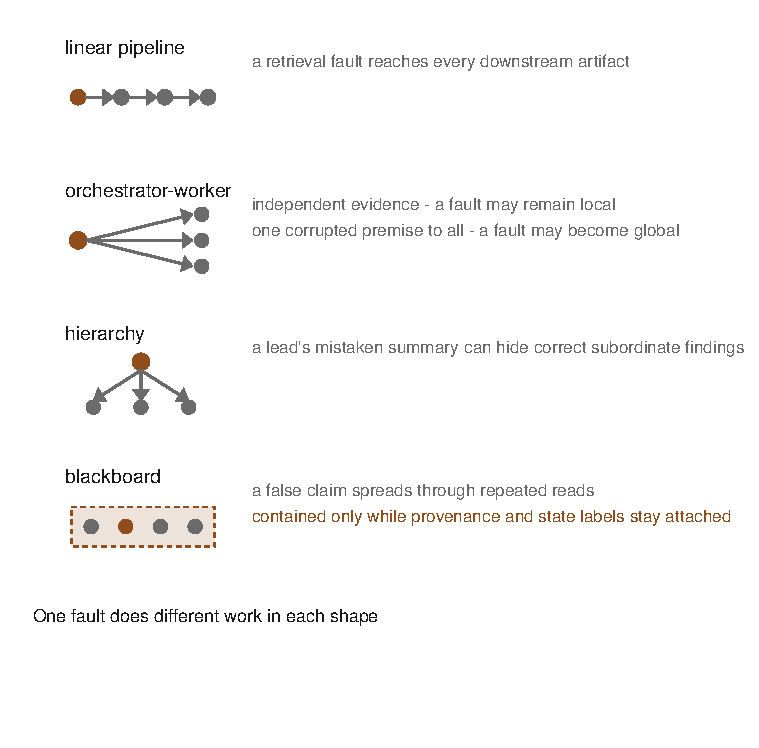
\includegraphics[keepaspectratio,alt={Fault propagation depends on collaboration topology, ranging from downstream contamination in pipelines to contained local errors when shared systems preserve provenance and state labels.}]{figures/ch17-topology-faults.pdf}}
\caption{Fault propagation depends on collaboration topology, ranging from downstream contamination in pipelines to contained local errors when shared systems preserve provenance and state labels.}
\end{figure}

Containment is conditional. A shared corrupted premise, an inaccurate lead summary, or repeated reads of an unqualified claim can turn a local error into a global one.

\Needspace{5\baselineskip}

Observation routes are therefore part of correctness. Record:

\begin{itemize}
\tightlist
\item
  which workers see raw tool output;
\item
  which receive only summaries;
\item
  whether a downstream component can request new upstream evidence;
\item
  whether workers see others' tentative conclusions before forming their own;
\item
  where contradictory results converge; and
\item
  which component can mark shared state disputed or invalid.
\end{itemize}

These properties govern error correlation, recovery, and attribution even when every worker uses the same model and prompt.

Runtime oversight can represent the topology as an interaction graph whose nodes are workers and artifacts and whose edges are messages or state transitions. That representation is a thinly supported companion idea and has not been validated as a monitoring standard. It remains a useful inspection tool because it exposes unreachable reviewers, unexpected broadcasts, and missing convergence paths.

Topology should be tested through faults, not inferred from diagrams.

\Needspace{5\baselineskip}

For a pipeline:

\begin{itemize}
\tightlist
\item
  remove or corrupt one stage output;
\item
  verify that downstream work stops or marks the state incomplete;
\item
  test whether the pipeline can widen or restart upstream.
\end{itemize}

\Needspace{5\baselineskip}

For an orchestrator-worker system:

\begin{itemize}
\tightlist
\item
  delay one worker;
\item
  inject contradictory findings;
\item
  corrupt one worker's input;
\item
  verify that the orchestrator distinguishes missing, late, and conflicting evidence.
\end{itemize}

\Needspace{5\baselineskip}

For a hierarchy:

\begin{itemize}
\tightlist
\item
  insert a critical minority finding at a subordinate level;
\item
  verify that it survives summarization;
\item
  test whether the lead can request source evidence.
\end{itemize}

\Needspace{5\baselineskip}

For a blackboard:

\begin{itemize}
\tightlist
\item
  submit conflicting updates;
\item
  verify that provenance and ordering remain attached;
\item
  preserve unresolved status rather than allowing last-write-wins to manufacture agreement.
\end{itemize}

The strongest evidence here, from Jia et al., concerns synthetic injected faults. Naturally occurring production faults lie outside that result, and the injected fault distribution determines what the comparison can show.

The reported closed-loop advantage supplies a reason to run local fault tests. It does not remove their necessity.

\Needspace{5\baselineskip}

The acceptable topology is the simplest one that:

\begin{itemize}
\tightlist
\item
  preserves the evidence the task requires;
\item
  contains representative faults;
\item
  exposes incomplete and disputed state;
\item
  keeps aggregation failures observable; and
\item
  clears the live single-agent gate on the target workload.
\end{itemize}

\section{Dispatch only work whose dependencies are satisfied}\label{dispatch-only-work-whose-dependencies-are-satisfied}

In a narrative reconstruction from my workflow harness, six planned work items initially appeared ready to run together. A pre-dispatch overlap check showed that four touched the same adapter file and its test. The schedule therefore became two waves. Three items could run in parallel, including two disjoint changes and one low-risk item from the colliding group. The remaining three ran sequentially in increasing risk order.

The scheduler selected a maximum independent set of nonconflicting work. Maximizing the number of simultaneous workers was not the objective.

The work-item identities, overlap matrix, and dispatch log from that sweep were not preserved, so the example illustrates the scheduling decision without providing an auditable result. The evidence for dynamic task graphs is also directional. The example cannot strengthen it.

A \textbf{dependency graph} represents units of work as nodes and prerequisites or conflicts as edges. It becomes a \textbf{task graph} when the runtime uses those records to decide which nodes are eligible for dispatch. A node becomes ready only when its prerequisites have completed successfully and its declared resources do not conflict with another running node. Independent work need not wait behind an unrelated serial step.

Execution can also change which work exists. A repository investigation may begin with one node that locates the affected adapter, then create package-specific repair nodes only after the adapter is identified. A failed compatibility check may add a migration node and block integration. A fixed schedule must either predict those branches in advance or leave workers idle while a central planner reconstructs dependencies from messages.

Dynamic dispatch does not mean unconstrained autonomy. The runtime performs a mechanical transition from \texttt{blocked} to \texttt{ready} when explicit conditions become true. Semantic decisions, such as whether a test failure warrants a new task, still require a model or person to propose the node and its dependencies. The scheduler validates that record and executes it under policy.

Yu et al.~(\href{https://arxiv.org/abs/2503.07675}{2025}) provide the only direct systems report attached to this practice, at directional strength. DynTaskMAS contains no controlled comparison between dynamic and fixed scheduling. The study compared parallel with serial execution on one seven-agent travel-planning workload. It did not compare a dynamic schedule with a fixed parallel schedule or isolate the task graph from the asynchronous execution engine.

The reported improvement therefore shows only that parallel execution outperformed serial execution in that setting. It does not show that dynamic scheduling outperformed a well-designed fixed schedule.

Rose et al.~(\href{https://arxiv.org/abs/2605.15132}{2026}) in APWA, Luo et al.~(\href{https://arxiv.org/abs/2502.13965}{2025}) in Autellix, and Masters et al.~(\href{https://arxiv.org/abs/2510.02557}{2025}) in the Manager Agent research challenge provide separate directional examples of related planning and scheduling architectures. None replicates a dynamic-versus-fixed comparison.

No controlled result in the cited evidence establishes that a dynamic dependency graph improves repository work relative to a fixed schedule.

The narrower systems argument applies when dependencies vary during execution. If independent branches exist, their prerequisites are observable, and their durations are uncertain, an explicit graph can expose safe concurrency without forcing unrelated work through one serial queue. If the workflow is short, fixed, and inexpensive, a graph scheduler may add persistence and recovery complexity without creating useful parallelism.

Dependency accuracy is the central risk. A missing edge can dispatch two workers that edit the same file, migrate the same schema, or invalidate each other's assumptions. A false edge serializes work that could safely overlap.

\Needspace{5\baselineskip}

File overlap is only one conflict signal. Work may also conflict through:

\begin{itemize}
\tightlist
\item
  generated artifacts;
\item
  shared test fixtures;
\item
  database schemas;
\item
  deployment environments;
\item
  locks or leases;
\item
  external services;
\item
  mutable caches; or
\item
  logical invariants spanning disjoint files.
\end{itemize}

Each node therefore needs enough state to support both scheduling and recovery:

\begin{verbatim}
node_id: stable logical identity
inputs: immutable artifact versions
depends_on: prerequisite nodes that must succeed
conflicts_with: resources or nodes that cannot overlap
owner: currently assigned worker
attempt: retry identity
status: blocked | ready | running | succeeded | failed
outputs: versioned artifacts and supporting evidence
\end{verbatim}

The attempt identity prevents a late response from an expired worker from overwriting a successful retry. Immutable input versions reveal when a ready node was planned against stale state. Versioned outputs allow downstream nodes to distinguish attempts that produced different artifacts.

These requirements come from the execution topology. Drawing the graph supplies none of them.

In my workflow harness, notification-driven dispatch ends the coordinating turn after work is assigned and resumes it when completion events arrive. This avoids a polling loop that consumes attention while no state has changed. Mechanical parallel-set detection checks dependency layers, blocking edges, and overlapping file paths.

Those rules illustrate the mechanism. They do not provide comparative performance evidence.

A per-step time limit contains a slow or failed worker only when expiration produces and propagates a real failure. Treating a timeout as success destroys the evidence of failure and may release downstream nodes without their required inputs. The schedule then appears healthy because it erased the event needed to diagnose it.

Dispatch should fail closed:

\begin{verbatim}
worker exceeds time limit
    -> attempt fails visibly
    -> dependent nodes remain blocked
    -> retry, escalation, or cancellation policy runs
\end{verbatim}

Retries require the same discipline. A retry creates a new attempt for the same logical node rather than a second independent task. The scheduler must either establish that repeated execution is idempotent or isolate side effects before trying again. Otherwise a timeout can produce duplicate comments, partial writes, or two workers claiming the same resource.

\Needspace{5\baselineskip}

Dynamic graphs are most useful when they expose decisions that were previously implicit. The runtime should be able to explain:

\begin{itemize}
\tightlist
\item
  why a node remains blocked;
\item
  which successful output released it;
\item
  which conflict prevents concurrent execution;
\item
  which attempt currently owns it;
\item
  which input version it was planned against; and
\item
  why a failure created, removed, or blocked another node.
\end{itemize}

If those answers cannot be reconstructed, the graph has become another hidden coordinator rather than an observable allocation mechanism.

\section{Promote topology from a recorded comparison}\label{promote-topology-from-a-recorded-comparison}

A structural redesign should end in a reproducible allocation decision. A diagram and a promising demonstration are not enough. The following protocol is narrow enough to apply to an existing workflow while preserving the distinctions developed in this chapter.

\section{1. Select one persistent failure class}\label{select-one-persistent-failure-class}

Use repeated paired runs across the current and upgraded model configurations. Preserve the first-upstream-failure assignment from Chapter 10.

Do not begin from a broad objective such as ``improve collaboration.'' Name the failure class whose path the structural change is expected to interrupt.

\section{2. Draw the current causal path}\label{draw-the-current-causal-path}

\Needspace{5\baselineskip}

Mark:

\begin{itemize}
\tightlist
\item
  where evidence originates;
\item
  where interpretation occurs;
\item
  where state becomes durable;
\item
  where authority changes hands;
\item
  where verification occurs; and
\item
  where the final decision converges.
\end{itemize}

Identify the smallest boundary at which the target failure could have become observable and stoppable.

\section{3. Preserve the live single-agent baseline}\label{preserve-the-live-single-agent-baseline}

\Needspace{5\baselineskip}

Replay the existing single-agent workflow on the current golden set. Record:

\begin{itemize}
\tightlist
\item
  pass\textsuperscript{k} or the selected reliability measure;
\item
  the chosen cost axis;
\item
  elapsed time;
\item
  tool and model use;
\item
  failures by class; and
\item
  the complete configuration identity.
\end{itemize}

Keep this baseline executable for later model releases. A topology should not receive permanent credit from a comparison against an obsolete single-agent system.

\section{4. Specify one structural treatment}\label{specify-one-structural-treatment}

\Needspace{5\baselineskip}

The treatment may be:

\begin{itemize}
\tightlist
\item
  a deterministic verification loop;
\item
  a specialized role;
\item
  a structured handoff;
\item
  a different communication topology;
\item
  a new aggregation rule; or
\item
  a dependency-aware dispatcher.
\end{itemize}

State which boundary changes and which causal path the change is expected to interrupt. Avoid combining several architectural changes unless the experiment is explicitly evaluating the combined system.

\section{5. Record the promotion rule before execution}\label{record-the-promotion-rule-before-execution}

\Needspace{5\baselineskip}

The rule should include:

\begin{itemize}
\tightlist
\item
  a task-success floor;
\item
  a reliability requirement;
\item
  a cost ceiling;
\item
  a latency limit where relevant;
\item
  a mechanism condition; and
\item
  any required fault-containment result.
\end{itemize}

A mechanism condition might require at least one delegated result to be consumed by the aggregator or require the scheduler to dispatch at least one pair of independent nodes concurrently. When candidates are voted on or synthesized, add a check for whether an oracle-correct candidate was retained or discarded.

\section{6. Inject a representative fault}\label{inject-a-representative-fault}

\Needspace{5\baselineskip}

Choose a fault matched to the proposed structure:

\begin{itemize}
\tightlist
\item
  For a pipeline, corrupt or omit an upstream artifact.
\item
  For an orchestrator, delay one worker or return contradictory findings.
\item
  For a hierarchy, place a critical result in a minority branch.
\item
  For a blackboard, submit conflicting updates and inspect ordering and provenance.
\item
  For a task graph, omit a dependency, introduce a false conflict, expire a worker attempt, or return a late completion.
\end{itemize}

Verify that incomplete or disputed state remains visible and that downstream work does not proceed as though the missing evidence existed.

\section{7. Run paired repeated trials}\label{run-paired-repeated-trials}

Run baseline and treatment on the same task versions. Keep the model, harness, permissions, evaluator, and execution environment fixed except for the declared structural change.

\Needspace{5\baselineskip}

Report separately:

\begin{itemize}
\tightlist
\item
  correctness;
\item
  reliability;
\item
  latency;
\item
  total computation;
\item
  monetary or token cost;
\item
  coordination failures;
\item
  usability or review burden; and
\item
  target failure-class frequency.
\end{itemize}

Inspect traces to confirm that delegation, scheduling, coordination, and aggregation actually occurred. A configured mechanism that never enters the execution path has not been evaluated.

\section{8. Promote, retain, or redesign}\label{promote-retain-or-redesign}

Promote only when the treatment clears the recorded success, reliability, cost, mechanism, and fault-containment conditions.

Retain the baseline when additional structure does not earn its coordination cost.

Redesign when the trace shows that the treatment changed a boundary but left the target failure path intact. The next experiment may require a narrower specialist role, another handoff field, a different aggregation rule, a corrected dependency model, or no additional worker.

The resulting record should be understandable without trusting the architecture's name. Promotion depends on whether the observed execution supports the claimed benefit, not on whether the design can be described as dynamic, hierarchical, multi-agent, or dependency-aware.

\section*{Sources and evidence}

The evidence grouping on each entry below comes from its catalog record. Author-system cases in this chapter are narrative illustration and are not part of the evidence base.

\begin{itemize}
\tightlist
\item
  Bertalani\v{c}, et al.~2026. \emph{The Cost of Consensus}. arXiv:2605.00914. Exploratory evidence on aggregation failure; Chapter 5 carries the reported oracle-gap result.
\item
  Böckeler, Birgitta. 2026. ``Harness Engineering.'' MartinFowler.com, February 17. Practitioner account based partly on vendor-reported Codex-team practice.
\item
  Cemri, M., et al.~2025. ``Why Do Multi-Agent LLM Systems Fail?'' arXiv:2503.13657. MAST failure taxonomy and benchmark-framework interventions.
\item
  Chun, Jina, et al.~2025. ``Is Multi-Agent Debate the Silver Bullet?'' arXiv:2503.12029. Audit-retained strong evidence on debate performance against task baselines; reports inference cost across debate variants and leaves the single-model cost comparison open.
\item
  Huang, Jia, and Joey Tianyi Zhou. 2026. ``A Two-Dimensional Framework for AI Agent Design Patterns: Cognitive Function and Execution Topology.'' arXiv:2605.13850. Directional taxonomy of topology choices.
\item
  Jia, J., et al.~2026. ``MAS-FIRE: Fault Injection and Reliability Evaluation for LLM-Based Multi-Agent Systems.'' arXiv:2602.19843. Synthetic fault injection across three architectures.
\item
  Jain, Prateek. 2026. ``Harness Engineering: The New DevOps Layer for AI Agents.'' r/devops, May 27. Anecdotal practitioner account.
\item
  Kim, T., et al.~2026. ``Why Do AI Agents Systematically Fail at Cloud Root Cause Analysis?'' arXiv:2602.09937. OpenRCA evidence on failure persistence across capability tiers and protocol intervention.
\item
  Kumar, et al.~2026. \emph{AgentForge}. arXiv:2604.13120. Directional evidence on multi-agent design.
\item
  Li, et al.~2026. \emph{SIMAS}. arXiv:2606.00655. Audit-retained strong evidence on token cost, non-monotonic scaling, and debate versus self-correction.
\item
  Luo, et al.~2025. \emph{Autellix}. arXiv:2502.13965. Directional scheduling and orchestration example.
\item
  Masters, et al.~2025. \emph{Manager Agent research challenge}. arXiv:2510.02557. Directional planning and scheduling example.
\item
  Qian, et al.~2024. \emph{MacNet}. arXiv:2406.07155. Directional evidence on network scaling.
\item
  Rose, Evan, et al.~2026. \emph{APWA: A Distributed Architecture for Parallelizable Agentic Workflows}. arXiv:2605.15132. Directional orchestration example.
\item
  Shang, Wenlong. 2026. \emph{``Theater of Mind'' for LLMs: A Cognitive Architecture Based on Global Workspace Theory}. arXiv:2604.08206. Directional blackboard and global-workspace design; single-author architecture proposal, not a controlled measurement.
\item
  Tian, et al.~2025. ``Beyond the Strongest LLM.'' arXiv:2509.23537. Directional evidence on multi-agent teams.
\item
  Yu, Junwei, Yepeng Ding, and Hiroyuki Sato. 2025. \emph{DynTaskMAS}. arXiv:2503.07675. Directional parallel-versus-serial result on a seven-agent travel-planning workload; no controlled dynamic-versus-fixed comparison.
\item
  Zhao, et al.~2026. \emph{ATOM}. arXiv:2605.26178. Audit-retained strong evidence on difficulty-conditioned topology across six short-form benchmarks.
\end{itemize}

\textbf{Author-system illustration cited inline}

\begin{itemize}
\tightlist
\item
  Not an evidence item: CodeProbe, the author's task-mining evaluation tool, \href{https://github.com/sjarmak/codeprobe}{public repository}. Named inline for the preamble rerun described in the opening, which is narrative illustration.
\end{itemize}
